\chapter{GENERAL SCOPE OF THE PROJECT}

\section*{Introduction}
\addcontentsline{toc}{section}{Introduction}
In this chapter, we will begin by defining the project in its practical and theoretical framework. We will present our host organization by detailing its organizational chart and architecture. Subsequently, we will describe the state of the art as well as the problem and limitations of the existing solution. Finally, we will outline the proposed solution.


In this chapter, I will present my project in general terms, setting out the project framework, then looking at the existing situation and the solutions to be provided. Finally, I will present the working methodology adopted for this project.

\section{Project Framework}

I will start by introducing my host organization, which is where my project took place.

\subsection{General presentation of the host organization}

BMG, a consulting firm and publisher of customized and innovative digital solutions, launched in January 2018, whose business is:
\begin{itemize}
    \item Helping customers formalize and implement their digital transformation projects.
    \item Supporting economic players and NGOs in the design and implementation of their digital projects, through a targeted consulting and support approach that takes into account human capital and structures the present and makes it evolve in line with the organization's digital strategy.
\end{itemize}

\subsection{Organization chart}

The following figure illustrates the organizational chart of the host organization, providing a clear representation of its structure and hierarchy.

\begin{figure}[h]
    \centering
    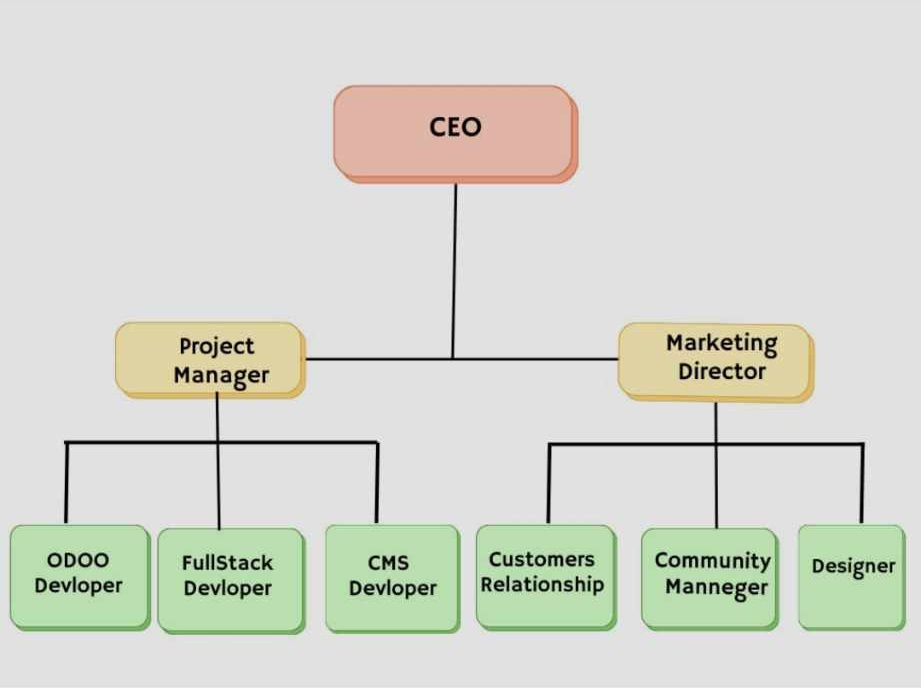
\includegraphics[width=1\textwidth]{media/org.jpg}
    \caption{Organizational chart of the host organization}
    \label{fig:Organizational chart of the host organization}
\end{figure}

\begin{itemize}
    \item Development of collaborative platforms
    \item Mobile development
    \item Web development
    \item E-commerce and marketplaces
    \item SEO and optimization
    \item ERP integration
    \item Data analysis
\end{itemize}


\section{Project Context}

An Enterprise Resource Planning (ERP \cite{erp})  system manages and monitors all information and operational services of a company.

To qualify as an "integrated management software," an ERP must adhere to two fundamental principles:

\begin{itemize}

    \item Building computer applications as independent but compatible modules on a single database.
    \item Using a workflow engine to define tasks and manage their realization across all necessary modules.

    \item Integration: ERP brings together data and processes from different departments into a single platform, avoiding data duplication and facilitating collaboration.

    \item Centralization: ERP provides a real-time overview of the company by centralizing information in a single database, enabling faster and more informed decision-making.
\end{itemize}

In summary, integration and centralization are fundamental ERP principles that optimize company management by unifying information and processes and providing real-time insights.


\subsection{Advantages of Choosing Odoo}

Odoo was selected for its:

\begin{itemize}
    \item Comprehensive Solution: Odoo integrates various business functions like CRM, accounting, and inventory, simplifying management.
    
    \item Flexibility and Customization: Odoo's modular architecture allows easy customization to suit specific needs.
    
    \item Cost-Effectiveness: Odoo's community edition offers competitive pricing with no licensing fees.
    
    \item Strong Community Support: Odoo has a large community of developers and users, providing extensive support and regular updates.
    
    \item User-Friendly Interface: Odoo's clean and intuitive interface enhances user experience, facilitating navigation and feature utilization.
\end{itemize}

\subsection{Advantages of Choosing Odoo for the Project}

Odoo offers several advantages specifically suited to your project needs:

\begin{itemize}
    \item Tailored Solution: Odoo's modular architecture allows for customization to specifically address the requirements of your project, ensuring a tailored solution.
    
    \item Integration Capabilities: With its comprehensive suite of integrated modules, Odoo facilitates seamless integration of various business functions, streamlining project management processes.
    
    \item User-Friendly Interface: Odoo's intuitive interface enhances user experience, enabling smooth navigation and efficient utilization of project management features by your team.
\end{itemize}


\subsection{Project Overview}

Today, companies want to embrace new technologies and use them to be more efficient, hence integrating comprehensive, configurable, and flexible management solutions for handling everything related to their business. This step is crucial to have a clear idea of the existing situation by analyzing it, then formulating an action plan and subsequently conducting a review focusing on weaknesses.

\subsection{Analysis of the Existing System}

The current Odoo rental application exhibits various shortcomings affecting operational efficiency:
\begin{itemize}
    \item Lack of centralized data management leads to data fragmentation and inconsistencies.
    \item Inadequate communication tools result in delays and misunderstandings.
    \item Limited customization options restrict adaptation to unique business needs.
    \item Reporting features are insufficient for real-time insights into operations.
\end{itemize}

\subsection{Critique of the Existing System}

Critiques of the existing Odoo rental app:
\begin{itemize}
    \item Decentralized data storage causes inefficiencies and inaccuracies.
    \item The lack of integrated communication tools leads to coordination issues.
    \item Limited customization hampers adaptation to specific business requirements.
    \item Inadequate reporting capabilities hinder real-time decision-making.
\end{itemize}

\section{Proposed Solution}

Our proposed solution involves the development of a customized rental management system tailored to your specific business needs. This system will offer a user-friendly interface, facilitating seamless control and monitoring of rental operations. By centralizing data management and integrating communication tools, our solution aims to enhance operational efficiency and customer satisfaction.

Key features of our proposed solution include:

\begin{itemize}
    \item Centralized data management to eliminate fragmentation and 
\\ inconsistencies.
    \item Integration of communication tools for improved coordination and client engagement.
    \item Extensive customization options to align the system with your unique business requirements.
    \item Advanced reporting features for real-time insights into rental operations.
\end{itemize}


Before detailing the improvements, the following table \ref{tab:comparison}  provides a comparison between the existing rental Odoo app and the proposed rental Odoo app, highlighting key differences and enhancements.

\begin{table}[h]
\centering
\resizebox{\textwidth}{!}{
\begin{tabular}{|p{3.5cm}|>{\centering\arraybackslash}p{5.5cm}|>{\centering\arraybackslash}p{5.5cm}|}
\hline
\rowcolor{purple!20} \diagbox[dir=NW]{\textbf{Feature}}{\textbf{Systems}} & \textbf{Existing Rental Odoo App} & \textbf{Proposed Rental Odoo App} \\
\hline
\hline
Centralized Data Management & Decentralized data management & Centralized data management eliminates fragmentation and inconsistencies \\
\hline
Communication Tools & Limited communication tools & Integrated communication tools facilitate collaboration \\
\hline
Customization Options & Limited customization options & Extensive customization options for specific requirements \\
\hline
Reporting Features & Insufficient reporting features & Advanced reporting for real-time insights \\
\hline
User Interface & May lack intuitiveness & User-friendly interface for ease of use \\
\hline
Workflow Automation & Minimal workflow automation & Robust workflow automation for process optimization \\
\hline
Scalability & Limited scalability & Scalable architecture for business growth \\
\hline
Customer Support & Limited customer support & Comprehensive customer support for implementation and usage \\
\hline
Integration Capabilities & Limited integration & Seamless integration with other systems \\
\hline
Security & Insufficient security measures & Robust security features for data protection \\
\hline
\end{tabular}
}
\caption{Comparison between Existing and Proposed Rental Odoo Apps}
\label{tab:comparison}
\end{table}
\newpage
\section{Methodology and Modeling Framework Adopted}


The selection of a methodology depends on the project's nature and scale. For small, well-defined projects, a waterfall approach may suffice. However, for projects with evolving requirements, an iterative or prototyping methodology is preferable.

Among iterative methodologies, Agile \cite{agile} methods are widely adopted worldwide. Agile fosters collaboration and embraces incremental approaches, producing high-quality products while accommodating evolving client needs. Agile promotes continuous quality management and early issue detection, minimizing cost and schedule penalties.

The nature of our project, which is evolutionary and characterized by incomplete requirements, led us to adopt an Agile methodology, specifically SCRUM.

\subsection{Overview of SCRUM Methodology}


SCRUM \cite{scrum} methodology emphasizes incremental development through transparent management of evolving requirements. With frequent deliveries, typically every four weeks, clients receive functional software at the end of each iteration. As the project progresses, the software becomes more feature-rich. SCRUM relies on iterative development at a consistent pace to achieve project objectives.


\section{Modeling Language}


As a modeling language, I used the Unified Modeling Language (UML \cite{uml}). It is commonly used in all product projects and offers several diagrams that provide a computational representation of standard elements and real-world problems.


\section*{Conclusion}
\addcontentsline{toc}{section}{Conclusion}

In this chapter, I began by introducing the company, followed by an analysis and critique of the existing system. Based on this assessment, I proposed a solution that aims to address some of the observed issues. Finally, I discussed the choice of modeling language and the methodology adopted.

At this point, I can move on to the next chapter, which will focus on the planning and architecture of the project.
